% Implementation
\graphicspath{ {images/} }

This chapter discusses the platform and the programming techniques employed to
implement the application.  This application is a web application meant to run
on browser. Traditionally, Javascript or programing languages which transpile
to Javascript are employed to execute such web apps. 

In the implementation of this application a functional programming language
called Elm which transpiles to Javascript is used. Therefore, the chapter
starts with defending the benefits of using a functional programming in general
and also how Elm uses Model, View, Update architecture to implement a dynamic
front end.

Furthermore, it will be discussed how the Graph as a data-structure is defined. How
it is drawn on screen as SVG (Scalable Vector Graphics). How a function
generates a color palette for the coloring of the vertices. How vertices are
laid out in various geometrical patterns and how animations are implemented
among other things.


\section{Front End Development with The Elm Programming Language}

The project is developed using the Functional Programming paradigm. This is a
paradigm which has been in development and practice since the days of infancy
of computer science. Functional programming is based on a form of computation
called lambda calculus proposed by Alonzo Church. See \cite{Hudak2007}.

For most of the history of computing, functional programming remained in the
ivory towers of universities for purposes of exploring theoretical computer
science and language research.

In the last decades however, programming languages such as Haskell and a few
dialects of LISP have escaped the ivory towers to find application in the
software industry.

In this section we will discuss, why functional programming was chosen as the
programming paradigm of choice. How the functional programming language called
Elm is used to write a well organized, maintainable, intuitive and
understandable code to produce a dynamic front end.

\subsection{Why Functional Programming?}
Functional programming, makes the programmer think in a different way than what
may be called imperative programming. In the functional paradigm, functions are
first class citizens, which can be mashed up together in myriad different ways
such as the following -


\begin{enumerate}
\item A function given as input to a another function. 
\item A function producing another function as an output.
\item Composition of two functions dove-tailed to each other to produce another function.
\item Programming patterns being abstracted out as functions.
\end{enumerate}

For such Lego like usage of functions they must be dependable, such that for a
particular input a function will give a particular output just like
mathematical functions and has no business outside it's scope for side-effects.
With such confidence in the functions, they can be fitted with each other to
make them do complex computation. See \cite{Hughes89}.

Since the functional code is more reasonable and logical than imperative
programming the runtime errors are substantially less than imperative
programming and is easier to maintain.


\subsubsection{Separation of Concerns}
It may be asked that if functions don't have side effects, how do they print
output on the terminal or read file from the hard disk or accept inputs from a
user. Functional programming environments have a way of separating the pure
part of a program from the impure part, by introducing `actions'. These
`actions' or side-effects are treated as a form of encapsulated data, which
can be manipulated by pure functions, and the environment makes changes to the
outside world by executing these actions.

Therefore the programmer has to himself a large part of the program where he
deals with just pure functions. This allows him to exploit the perfectness of
pure functional programming.

This separation of concerns of pure and impure code in the context of the Elm
programming language is discussed in the \autoref{elm: architecture} called \emph{the Elm
Architecture}.

\subsection{Why Elm Programming Language for This Project?}

For the reasons in the previous sections, a functional programming language was chosen
keeping in mind that the size of this project would be quite substantial.
Unlike JavaScript, Elm does not require any external framework such as Angular
or React. This makes the program easier to reason with and maintainable.

Although, Elm is a new language which may not have as much community support as
JavaScript and it's various frameworks have, it has a compiler which gives
friendly error messages almost guiding the programmer for correct usage of the
language.

\subsection{The Elm Architecture}
\label{elm: architecture}
The Elm Architecture is a pattern of writing Elm code for responsive web applications. 
The architecture separates the concerns of front-end development into the following categories:

\begin{enumerate}
\item Model
\item View
\item Update
\end{enumerate}

The Model is a data structure which holds the state of a program. See
\cite{Fairbank19}. This state is used by the view function as an input to
render the webpage.  The webpage, when rendered has elements, which may trigger
events, such as user inputs by the way of clicking an HTML element. Such events
are caught by the Elm runtime and sent to the update function.  The update
function takes these event messages and changes the state. The changed state is
then rendered by the view function to a modified page.  Therefore, the Model is
changed by the update function, whereas it is used by the view function to
render a webpage according to a formula set by the programmer.


\section{Events as Messages}
\label{impl: messages}
The events described in section \autoref{elm: architecture} generated by
animation clocks and clicks of the user on graph elements and buttons, are
called messages in the Elm way of naming things. For this particular
application they are defined as an Algebraic Data Type as:

\begin{lstlisting}[language=elm
                  , caption={
                              Abstract Data Type Msg with it's Data Constructors.
                              These messages are emanated from buttons, graph vertices
                              system clocks and are received by the update function
                              to change the $Model$, which carries the state of the
                              program.
                  }
                  ]
type Msg
    = TimeDelta Float                  -- Clock Ticks for Animation
    | HoverOver Int                    -- Event when Mouse over a Vertex                              
    | MouseOut Int                     -- Event when Mouse out from a Vertex                               
    | VertexClicked Int                -- Event when Vertex Clicked                              
    | AnimationToggle                  -- Pause or Play Animation
    | AnimationStartOver               -- Restart Animation
    | ToggleVertexStatus Int           -- Select/Unselect Vertex
    | NextTopic                        -- Next Topic
    | PreviousTopic                    -- Previous Topic
\end{lstlisting}
The messages are not just generated by user interaction with this application,
they are are also generated by the animation clock as well as can be seen in
the first data constructor of the type $Msg$.
The clock ticks and the key strokes are events which initiate the update function to act on Model.
The animation clock and key presses need to be subscribed from the Elm runtime in the following way:

\begin{lstlisting}[language=elm
                  , caption={
                            Subscription of Animation clock and Key presses services.
                            Subscriptions are used to catch the events which are
                            emanated outside the DOM. In this code, a system clock
                            and key presses are subscribed to by the program.
                            }
                  ]
subscription : Model -> Sub Msg
subscription _ =
    Sub.batch
        [ E.onAnimationFrameDelta TimeDelta
        , E.onKeyPress keyDecoder
        ]
\label{listing: subsciption}
\end{lstlisting}

% Block diagram
\begin{figure}[h] % ’ht’ tells LaTeX to place the figure ’here’ or at the top of the page
\centering % centers the figure
\begin{tikzpicture}
% tikz code goes here
   \node[state] (q1) {Isomorphism};
   \node[state, right of=q1] (q2) {MaxkCut};
   \node[state, right of=q2] (q3) {GraphColoring};
   \node[state, below of=q3] (q4) {VertexCover};
   \node[state, below of=q1] (q5) {TreeWidth};

   \draw (q1) edge[above, bend left] node{NextTopic} (q2)
         (q2) edge[below, bend left] node{PreviousTopic} (q1)
         (q2) edge[above, bend left] node{NextTopic} (q3)
         (q3) edge[below, bend left] node{PreviousTopic} (q2)
         (q3) edge[above, bend left] node{NextTopic} (q4)
         (q4) edge[below, bend left] node{PreviousTopic} (q3)
         (q4) edge[above, bend left] node{NextTopic} (q5)
         (q5) edge[below, bend left] node{PreviousTopic} (q4)
         (q5) edge[above, bend left] node{NextTopic} (q1)
         (q1) edge[below, bend left] node{PreviousTopic} (q5);
\end{tikzpicture}
\caption{This Finite State Machine (FSM) 
        shows how the messages, NextTopic and PreviousTopic
        changes the state of the program (the Model) from
        one topic to another. This is a subset of a much larger
        FSM in which the number of states and inputs are greater
        in number.
        }
\label{fig:my_label}
\end{figure}
% Block diagram
\section{Implementation of Graphs}
Inside the program, a graph exists as data structure which contains a list of
vertices and a list of edges. The vertex, as can be seen in \autoref{code: typeGraph} which is a data type defined
separately consists of a name (which is an integer), a color, a 2D position (it
is actually implemented using a 3D vector, with z is always kept at zero).  An
edge on the other hand is defined as a combination of two vertices. Such Graphs
are present in the Model in and are used by the view function to be drawn as
SVG.

\begin{lstlisting}[  language=elm, 
                     caption={
                              Definition of Vertex, Edge and Graph.  Vertex is
                              defined as a data structure which has a name as
                              an integer, a position as a 3 dimensional vector,
                              color, and a flag which depicts if it has been
                              selected by the user.  An Edge has two Vertices and
                              a Graph contains a list of Vertices and a list of
                              Edges.
                             }
                  ,  label={code: typeGraph}
                  ]

-- Definition of Vertex
type alias Vertex =
    { name : Int, pos : Vec3, color : Color, glow : Bool }

-- Definition of Edge
type alias Edge =
    { vertexOne : Vertex, vertexTwo : Vertex }

-- Definition of Graph
type alias Graph =
    { vertices : List Vertex, edges : List Edge }
\end{lstlisting}

\subsection{Grid}
In the program a Grid is a list of 3D vectors or in other words a list of
position for vertices, which can be taken as an input by certain functions to
construct graphs or change shapes of graphs. 

A list of Vertices, for example can be formed by combining together lists of
names, colors and a grid.

Grids are important in implementing animations. There is a function, for
example, which which take two grids and output a grid which is geometrically in
between the two grids.

\subsection{Using Linear algebra to Initialize Grids}
Linear algebra, in particular manipulation of vectors using Matrices has been
used to create interesting grids for the placement of vertices in the scene.
This includes rotation, scaling and translation of vectors to from polygonal
patterns. Functions were created to form polygon with $n$ geometric vertices
which prove very handy in producing grids for various geometries like
the one seen in Graph Ismoporphism and Max k Cut examples.

As a small example, here is a functional programming code in \autoref{code:
centroid} to find the centroid of of three position vectors. You can observe
how first two vectors are added on line 3, and then it is pipelined to addition
with a third vector, which is in turn pipelined to being scaled by $0.33$
(divided by $3.0$). This could have been achieved in a single line of code, but
Elm reserves operators like $+$, $-$, $*$ for only numbers and they can't be
overloaded to work for vectors.


\begin{lstlisting}[  language=elm
                  ,  caption={
                              Finding Centroid of Three Vertices. It logically starts with
                              vertex the addition of positions of vertices v1 and v2. The output
                              of which goes to the same function at line 4 albeit
                              partially applied to position of v3. The output, which is the 
                              summation of the position of the three vertices 
                              in turn is passed to a scale function which 
                              effectively divides it's
                              input vector by three. Hence the centroid emerges
                              out of the other end.
                             }
                  ,  label={code: centroid}
                  ]
findCentroidOfVertices : Vertex -> Vertex -> Vertex -> Vec3
findCentroidOfVertices v1 v2 v3 =
   Math.Vector3.add v1.pos v2.pos
   |> Math.Vector3.add v3.pos
   |> Math.Vector3.scale 0.333
\end{lstlisting}

\subsection{Creating Polygons}
Two dimensional computer graphics was used to create polygons to form the Grids
or subset of Grids for Graphs. Functional programming techniques such as mapping
over a list was employed to create such grids. 
The construction of a polygon proceeds like this:

\begin{enumerate}
\item A list of floats containing ones is created. 

\item Each is converted to an angle in radians corresponding
to the polar position of the vertex. 

\item This list of angles is then presented to
a function which maps a horizontal vector with unit length over this list
such that the unit vector is rotated with an angle equal to the angle in the
list giving rise to a list of rotated vectors.

\item This regular polygon with vertices at unit distance from it's center is
then scaled. The scaling factor for x is sometimes different from that of y.
Which enables squeezing of the polygon along any 2 dimensional direction.

\item Mixing such polygons come handy to create more complicated shapes.

\item The polygon is then translated to an appropriate position on the SVG screen.

\end{enumerate}

\subsection{Implementing Colors}
To have a list of neighboring colors acting as a color palette we work on the
Hue Saturation Lightness color space (HSl), mostly varying the hue just pass a
region in the spectrum of hues (First, Second or Third) and the number of
colors needed as an Integer. On a scale from $0.00$ to $1.00$, the first region
will produce hues ranging from $0.00$ to $0.33$, the second producing it from
$0.33$ to $0.66$ and the third producing it between $0.66$ to $1.00$.

\subsection{Edges}
Edges are defined as a combination of two vertices. Since they are drawn as a
straight line segment between the positions of the two vertices, they do not require
positional data associated explicitly for them. It is drawn out from the vertices,
they contain.

\begin{figure}[!ht]
\centering
\includegraphics[scale=0.047]{Graph1New}
\caption{
         Drawing a Graph. Starting with a grid of positions
         a set of vertices are created. Connecting the vertices,
         the edges are formed according to a list of tuples. The 
         vertices is then laid on top of the edges by concatenating list
         of SVG elements representing edges with list of SVG elements
         of Vertices. This is followed by this new list being concatenated
         with a list of SVG text representing the vertex names.
        }
\end{figure}

\section{Implementation of Animations}
In this section, it will be explained how various animations in the
application are implemented. Though there are minor differences between animations
for one topic to another, they follow a common pattern. The common pattern is
this that events are generated by a quasi-regular clock. These events trigger
the update function which transforms the current state of the program and
changes the position of certain abstract entities. The view function while
redrawing these entities takes the position information from the updated model
to draw them as SVG.

\subsection{Morphing Geometry of a Graph}
\label{animation: morphing}
In some of the animations in the application, the graph changes it's geometry
to visually look different than the original. This is accomplished by a
function which takes a graph and a grid to move the input graph incrementally
towards the grid with every tick of the animation clock. 
When the animation
is started, with each tick of the animation clock, the vertices of the
second graph move towards the target grid points with a constant velocity.
The velocity of a vertex is calculated by obtaining the displacement vector between
the target position and the current position of the vertex and also the time
available before the animation ends.
The displacement is calculated as $\vec{d} = \vec{p_t} - \vec{p_v}$, where
$\vec{p_t}$ is the target postion and $\vec{p_v}$ is the current position of
the vertex. The time available is calculated as $t = t_{available} -
t_{elapsed}$. The velocity is calculated as $\vec{v} = \vec{d}/t$.  The
distance the vertex must travel is hence calculated as $\Delta d = \vec{v}
\times \Delta t$.  Where $\Delta t$ is the time elapsed since the last tick of
the animation clock.


%PICTURE of Isomorphic Animation
\begin{figure}[h]
\centering
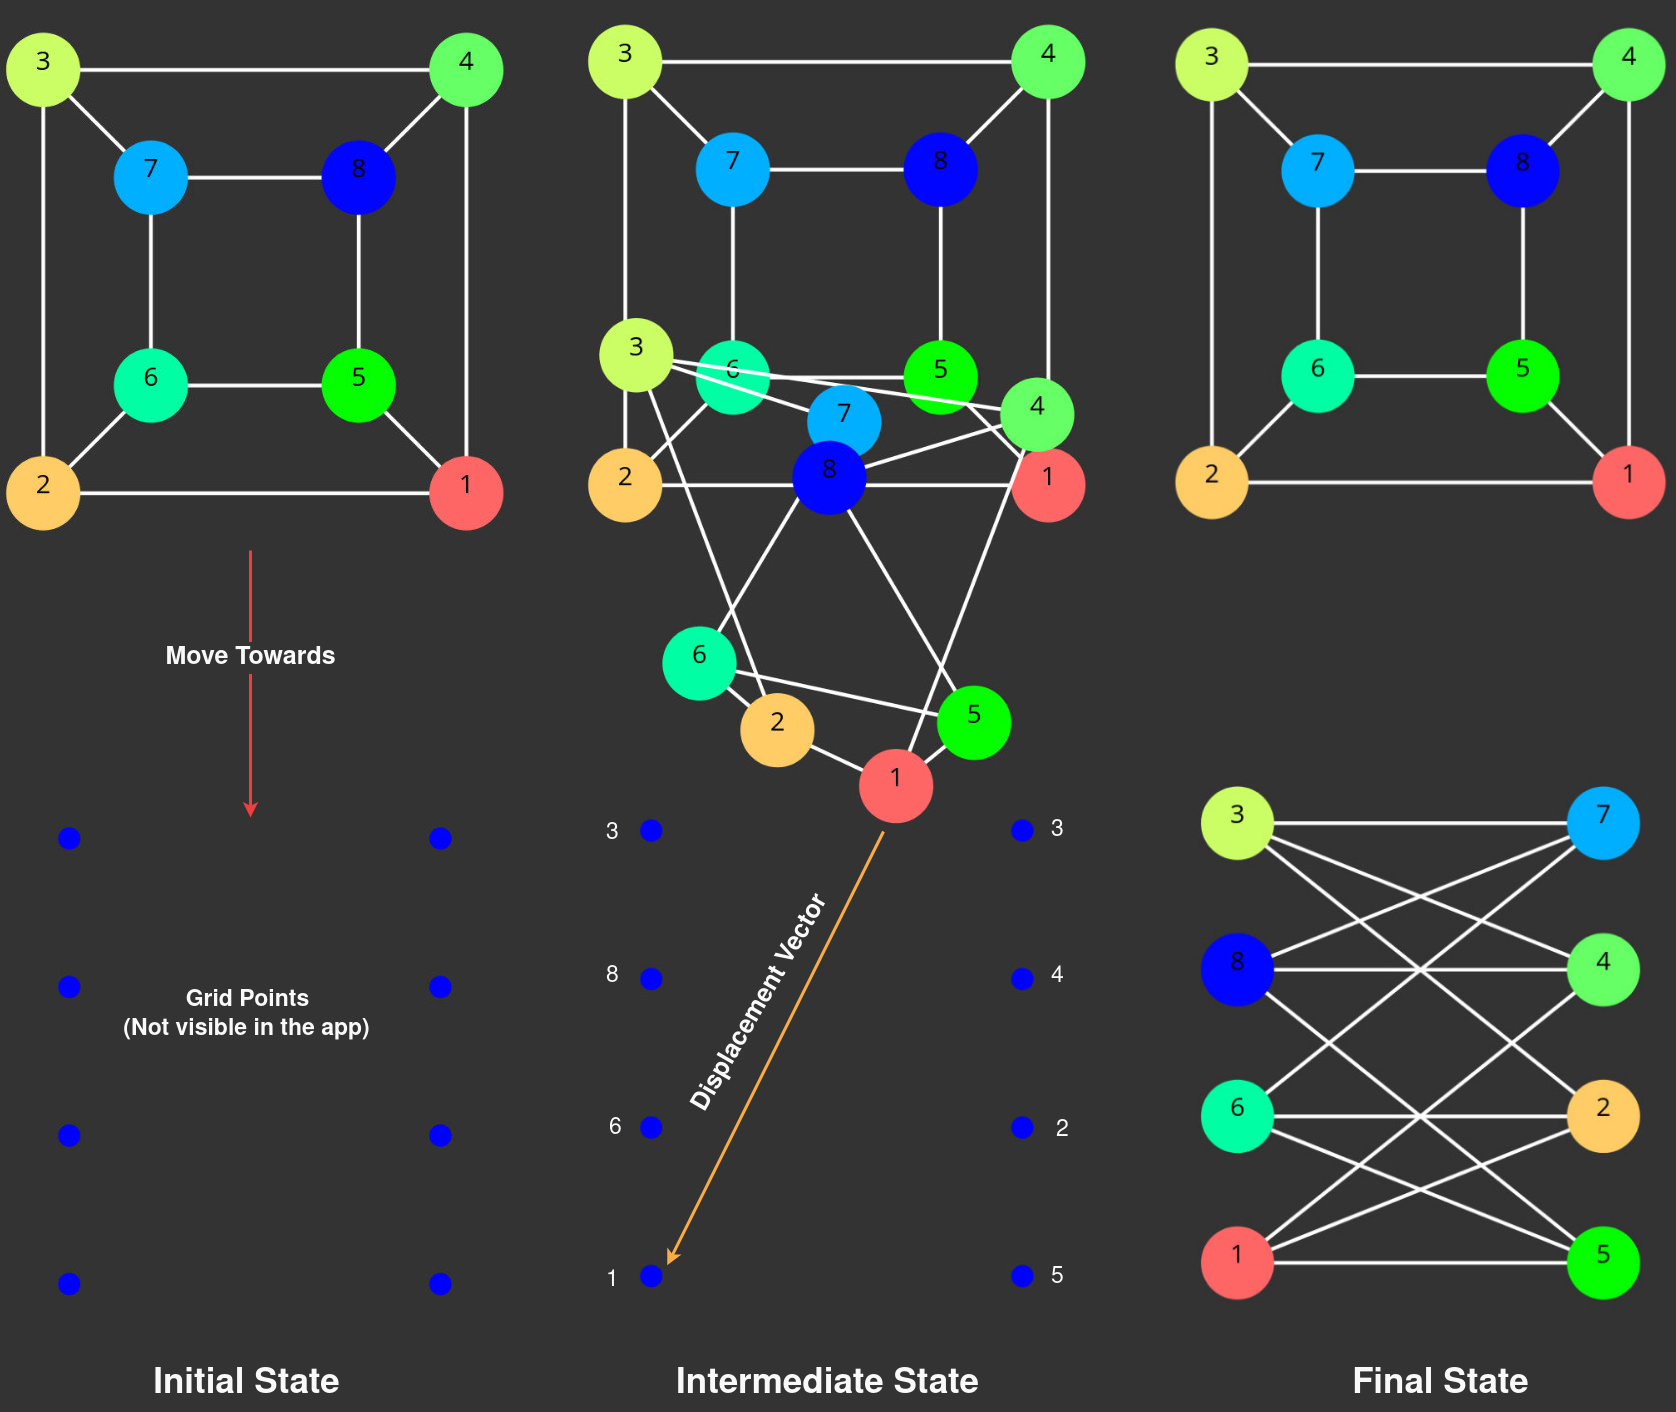
\includegraphics[width=4.22in]{IsomorphismAnimation}
\caption{
        Morphing a graph. This example from the Graph Isomorphism topic
        shows how shape transformation is done with the help of a targed grid.
        The target grid is shown as blue points.
        }
\label{animationfigure: isomorphism}
\end{figure}

\subsection{Re-formation of the Graphs}
At each tick of the animation clock the graph under transformation, is built
again, with vertices having the same name and color as the original but new
positions. The edges need to be re-constructed again as the vertex positions
have been renewed. This is something which is expected in the functional
programming paradigm where nothing is changed in place and new data structures
are created with application of a function. This is true not just for
animations, it is true for user-interaction or anything which requires visual
(Geometric or Color) modification of the graph.

The re-formation of the vertices and the edges are quite explicitly shown in
the Elm function shown in \autoref{code: morphGraph}. The function takes a
graph and a grid and produces a new graph situated at the new grid with new
vertices and edges.  The edges formed in the new graph are connected to the
same vertices (vertices with the same names, actually) as the original ones.

\begin{lstlisting}[language=elm, 
      caption={
      Changing the shape of a graph for animation.
      The first line, in the code describes the Type Signature of the function
      morphGraph. It says that the function takes a Graph and a Grid as input
      and produces a Graph as an output.
      The input Graph's vertices adopt the positions listed in the Grid.
   }
   , label={code: morphGraph}
   ]
morphGraph : Graph -> Grid -> Graph
morphGraph graph grid =
    let
        updatedVertices =
            List.map2 updatePositionVertex graph.vertices grid

        createEdge =
            updateEdge updatedVertices

        updatedEdges =
            List.map createEdge graph.edges
    in
    Graph updatedVertices updatedEdges

\end{lstlisting}

% Block diagram
\begin{figure}[ht] % ’ht’ tells LaTeX to place the figure ’here’ or at the top of the page
\centering % centers the figure
\begin{tikzpicture}
% tikz code goes here
   \node[state] (q1) {Initial Grid};
   \node[state, right of=q1] (q2) {Second Grid};
   \node[state, right of=q2, initial] (q3) {Penultimate Grid};
   \node[state, right of=q3] (q4) {Final Grid};

   \draw (q1) edge[above] node{TimeDelta} (q2)
         (q2) edge[draw=none] node{$\cdots$} (q3)
         (q2) edge[draw=none, above] node{TimeDelta(s)} (q3)
         (q3) edge[above] node{TimeDelta} (q4);
\end{tikzpicture}
\caption{ An FSM shows, how the animation progresses with
          each tick of the elm run-time clock, depicted as the message TimeDelta.
          With each such message the position of each vertex, takes their
          respective position in the following grid.
        }
\label{fig: animationFSM}
\end{figure}
\subsection{Drawing of Graphs}
Drawing graphs is done using SVG elements. The vertices are drawn as color
filled circles while the edges are drawn as straight line segments between the
positions of the related vertices. The edges are drawn first and the vertices
later so that vertices appear on top of the edges and the edges seem to be
appearing out of the surface of the vertices.

\section{Explanation Panel}

The Explanation Panel is the right half of each page concerned with a topic. 
It consist of the title of the topic and suggestions on how
to interpret and interact with the animations and user interactions.

The content of this panel depends on the state of the animation or the user
interaction associated with the topic.

The functions which populate the explanation panel with different elements have
therefore a subset of the \emph{Model} data-structure as it's input.  According
to the state of the program appropriate advises, instructions and buttons are
spawned on the panel.

The functions responsible for Explanation Panel in the case of user interaction
such as the ones in Graph Coloring and minimum vertex cover run a check on the
state of the program to know if the user is doing his task correctly. For
example in graph coloring, if two adjacent vertices are colored the same color,
there appears a message in the explanation panel warning about the same.

\section{Navigation and Control}
There are several buttons and keyboard shortcuts to go from one topic to the
next and to play/pause and restart animations. These have been implemented by
generating appropriate messages which are caught by the update function which
in turn updates the model (state of the program). The updated model of the
program is reflected on the screen by the view function.

\subsection{URL Management}
Although there is only one HTML page rendered (this application being a Single
Page Application), when the user navigates from one topic to another he can see
the URL path after the Website's name change to reflect the pseudo-page he is
on. This change in the URL is brought by the function $pushUrl$ at
appropriate situations.  The change in the URL is detected by the run-time to
produce the message $UrlChanged$ which in turn is caught by the Update function
to re-populate the page with new topic.

\subsection{Navigation Bar}
The navigation bar consists of buttons to go to the previous and the next
topics.  When the message $PreviousTopic$ or the message $NextTopic$ is
generated by the buttons respectively, the update function catches it to change
the state of the program (a data structure known as Model) to load it with the
details of the previous/next topic.

\subsection{Keyboard Shortcuts}
Keyboard shortcuts provide a fast way to test various functionalities while
developing the application.  These functionalities have not been taken away
even after development therefore they still can be used to trigger events in
the application. 
The key presses messages are registered by the elm run-time which in turn
triggers the update function to update the model. The updated model is now
rendered by the view function. Information about the keyboard shortcuts can be
availed on the screen by pressing the information icon present in the
navigation bar. Below is an example list of a few key-bindings.

\begin{itemize}
\item \textbf{p}: Toggle between pause and play animation. (Can be used instead of the Play/Pause button; Generates the $AnimationToggle$ message). \\
\item \textbf{r}: Restart animation. (Can be used instead of Restart Button; Generates the $AnimationStartOver$ message). \\
\item \textbf{n}: Go to the next topic. (Can be used instead of the navigation button; Generates the $NextTopic$ message). \\
\item \textbf{N}: Go to the previous topic. (Can be used instead of the navigation button; Generates the $PreviousTopic$ message). \\
\item \textbf{t}: Next animation (Can be used in case of Max k Cut and Tree width to go to the next animation; Generates the $NextAnimation$ message)
\end{itemize}

\section{Implementation of Topics}

\subsection{Graph Isomorphism}
\label{impl: isomporphism}

This topic is elucidated by a user interactive animation. Refer to
\autoref{story: isomorphism} for the details. The animation consists of two
Graphs which are the same. 

In the beginning the two graphs are superimposed with each other positionally.
Each graph is constructed by merging two polygons and connecting their vertices
in a wheel like structure.
As the animation begins one graph leaves it's position and transforms to
another shape.  This is achieved by instantiating the two graphs with same
position and form. An empty grid is also provided as the target set of
positions for the vertices of the second graph. 

When the animation is started, with each tick of the animation clock, the
vertices of the second graph move towards the target grid points with a
constant velocity. For the kinematics involved in this transition see
\emph{Morphing Geometry of a Graph} in \autoref{animation: morphing}.

For the user interaction part, when the user hovers over a vertex, or selects
it by pressing the corresponding numerical key on the keyboard, a Boolean
variable associated with the vertex is turned \emph{True}. A function filters
the list of vertices to find the selected vertex. Another function finds the
edges incident on the vertex and also the vertices adjacent to the selected
vertex by filtering over the list of edges in the graph. These are shown
differently in a highlighted color in both the graphs in the display section.
The explanation section also uses this data to explain how the selected vertex
is connected to the same adjacent vertices in both the graphs.

\subsection{Max k Cut}
\label{impl: maxkcut}
The Max k Cut topic has two animations back to back related to firstly the Max
2 Cut and then Max 3 Cut . See \autoref{story: maxkcut} for explanation of the
animations. The first animation has a graph constructed by merging two polygons.
The edges are so defined that the graph is nearly bipartite (see
\autoref{graphtheory: definitions} ) save for one edge (see \autoref{story:
max2cut}). The target grid for the animation is made of the combination of the
same polygons but set apart vertically. The kinematics of the animation is
executed the same way as is done for Graph Isomorphism.

The user can draw a predetermined line segment which seperates the two
sets. The line segment is superimposed by intersection points of the
line segments and the edges between the two sets. An intersection point
is calculated by finding intersection of two line segments. A linear algebra
library function was used for this task.

%%PICTURE of Max  2 Cut Animation
%\begin{figure}[h]
%\centering
%\includegraphics[width=3.50in]{max2cutAnimation}
%\caption{
%        Arrangement of animation of Max 2 Cut.
%        }
%\label{animationfigure: max2cut}
%\end{figure}

%PICTURE of Max  3 Cut Animation
\begin{figure}[h]
\centering
\includegraphics[width=4.22in]{max3cutanimation}
\caption{
        Arrangement of animation of Max 3 Cut.
        }
\label{animationfigure: max3cut}
\end{figure}
In the case of Max 3 Cut (see \autoref{story: max3cut}), the animation begins
with a tripartite graph. The graph is based upon a nonagon shaped grid. The
destination grid, in this animation is shape of an equilateral triangle, with
the grid points near the vertices of the said triangle. The graph consists of
three sets of vertices which settle down at the vicinity of the three vertices
of the equilateral triangle at the end of the animation. The kinematics of the
motion of the vertices is explained in \autoref{animation: morphing}.

\subsection{Graph Coloring}
The graph in this section is composed of two concentric pentagonal graphs such
that each vertex has three adjacent vertices. The user task is to color the
graph using three different colors. See \autoref{story: coloring} for further
explanation of the task.

When the user chooses a color from the color palette, the chosen color is
updated in the state of the program. When the user clicks a vertex, the color
of the vertex is changed with the color stored in the state of the program.

There is a function which makes a check while the user task is going on, whether
two adjacent vertices have similar color by doing a linear search on the edges.
If they are the information is used in the display to mark that edge differently
and a warning appears on the explanation panel based on this search.

If in a linear search for finding adjacent vertices of the same colors
doesn't have an output and if all the vertices have been colored, then
the function which populates text on the explanation panel shows a message that
the task is complete.

\subsection{Vertex Cover}

The graph in the Vertex Cover is based on composition of two square grids.

The user interaction for this topic asks the user to choose the minimum number
of vertices such that all the edges in the Graph belong to the set of vertices
which are incident on the chosen vertices. See \autoref{story: vertexcover}.

When the user clicks on a Vertex, there is a Boolean value associated with the
Vertex which becomes \emph{True}. There is a function which filters
the list of edges to find which of them have at least one of their vertices
\emph{selected}. Such edges are illuminated, for the user to note that the edge has
been covered.

There is another function which filters out the edges whose one of the vertices
have been selected, and yet another which counts the number of vertices which
have been selected.  When the all the edges have been covered, the program
checks for the number of vertices selected to do this by filtering the list of
vertices. In the case of the particular example in this project, the graph can
be covered using four vertices. Therefore if the number of vertices selected at
the end of the session are greater than four, then the explanation panel is
populated with a message that the task needs to be attempted again for proper
execution.

\subsection{Tree Width}
Tree width topic is implemented in a series of animations.  In the first
animation the vertices of the graph of this topic are arranged circularly
albeit with edges such that there is a cellular structure in present inherently
in the graph. This edges were set up in this graph by coding their connectivity
in a list of tuples.
This is also a graph-transition just like graph isomorphism. The target grid
for this transition is a regular lattice which reveals the cellular nature of
the graph. The kinematics of the transition is the same as that of graph
isomorphism (see \autoref{impl: isomporphism}) and Max k Cut (see
\autoref{impl: maxkcut}). For more information on the kinematics of such shape
transitions see \autoref{animation: morphing}.

The second part of the animation highlights one piece of the cellular structure
(see \autoref{}). The piece is also marked by drawing a blue dot at the center
of the it. The position of the blue dot is found by  taking the centroid of the
constituent vertices of the piece.

In the third part the centroid of all the pieces are found and marked as blue.
These blue dots are connected by special lines in the last part of the
animation to form the tree structure inherent in the original graph.

The animation series is followed step by step by explanation panel which responds
to the various states of the program.

\section{Modules}

The program is divided into ten modules.

The $Main$ module is of the central utility. It's function is to be a
starting point for the program and also to act as a porter to load the
functionality of individual graph theory topics to the state of the program
whenever the navigation commands demand so. 

The five topics included in the project own a module of their own. They are
$Isomorphism$, $Maxkcut$, $GraphColoring$, $VertexCover$ and $TreeWidth$ modules.
These modules are imported by the main function to be used on the screen.
Henceforth these will be collectively known as the \emph{Topic Modules}.

The $Graph$ module contains the data types and functions for representing,
constructing, drawing and animating the graphs. This module contains the most
geometry. This module is depended upon by all the \emph{topic modules}.

The $Explanation$ module contains the text data as a $0-nary$ functions
(functions which don't take input) used by topic modules for the explanation of
the respective topics. These only contain the definitions of the concerned
graph theory problems.

The $Messages$ module contains the messages which are generated with system
clock ticks or user interaction with the DOM elements.  Such messages are
defined as \emph{Algebraical Data Types} (see \autoref{impl: messages}) and are
imported by almost all other modules. This along with the $Main$ and $Graph$
modules form the central pillar of the program and are the minimum requirement
of the program to function.

%PICTURE of modules
\begin{figure}[h]
\centering
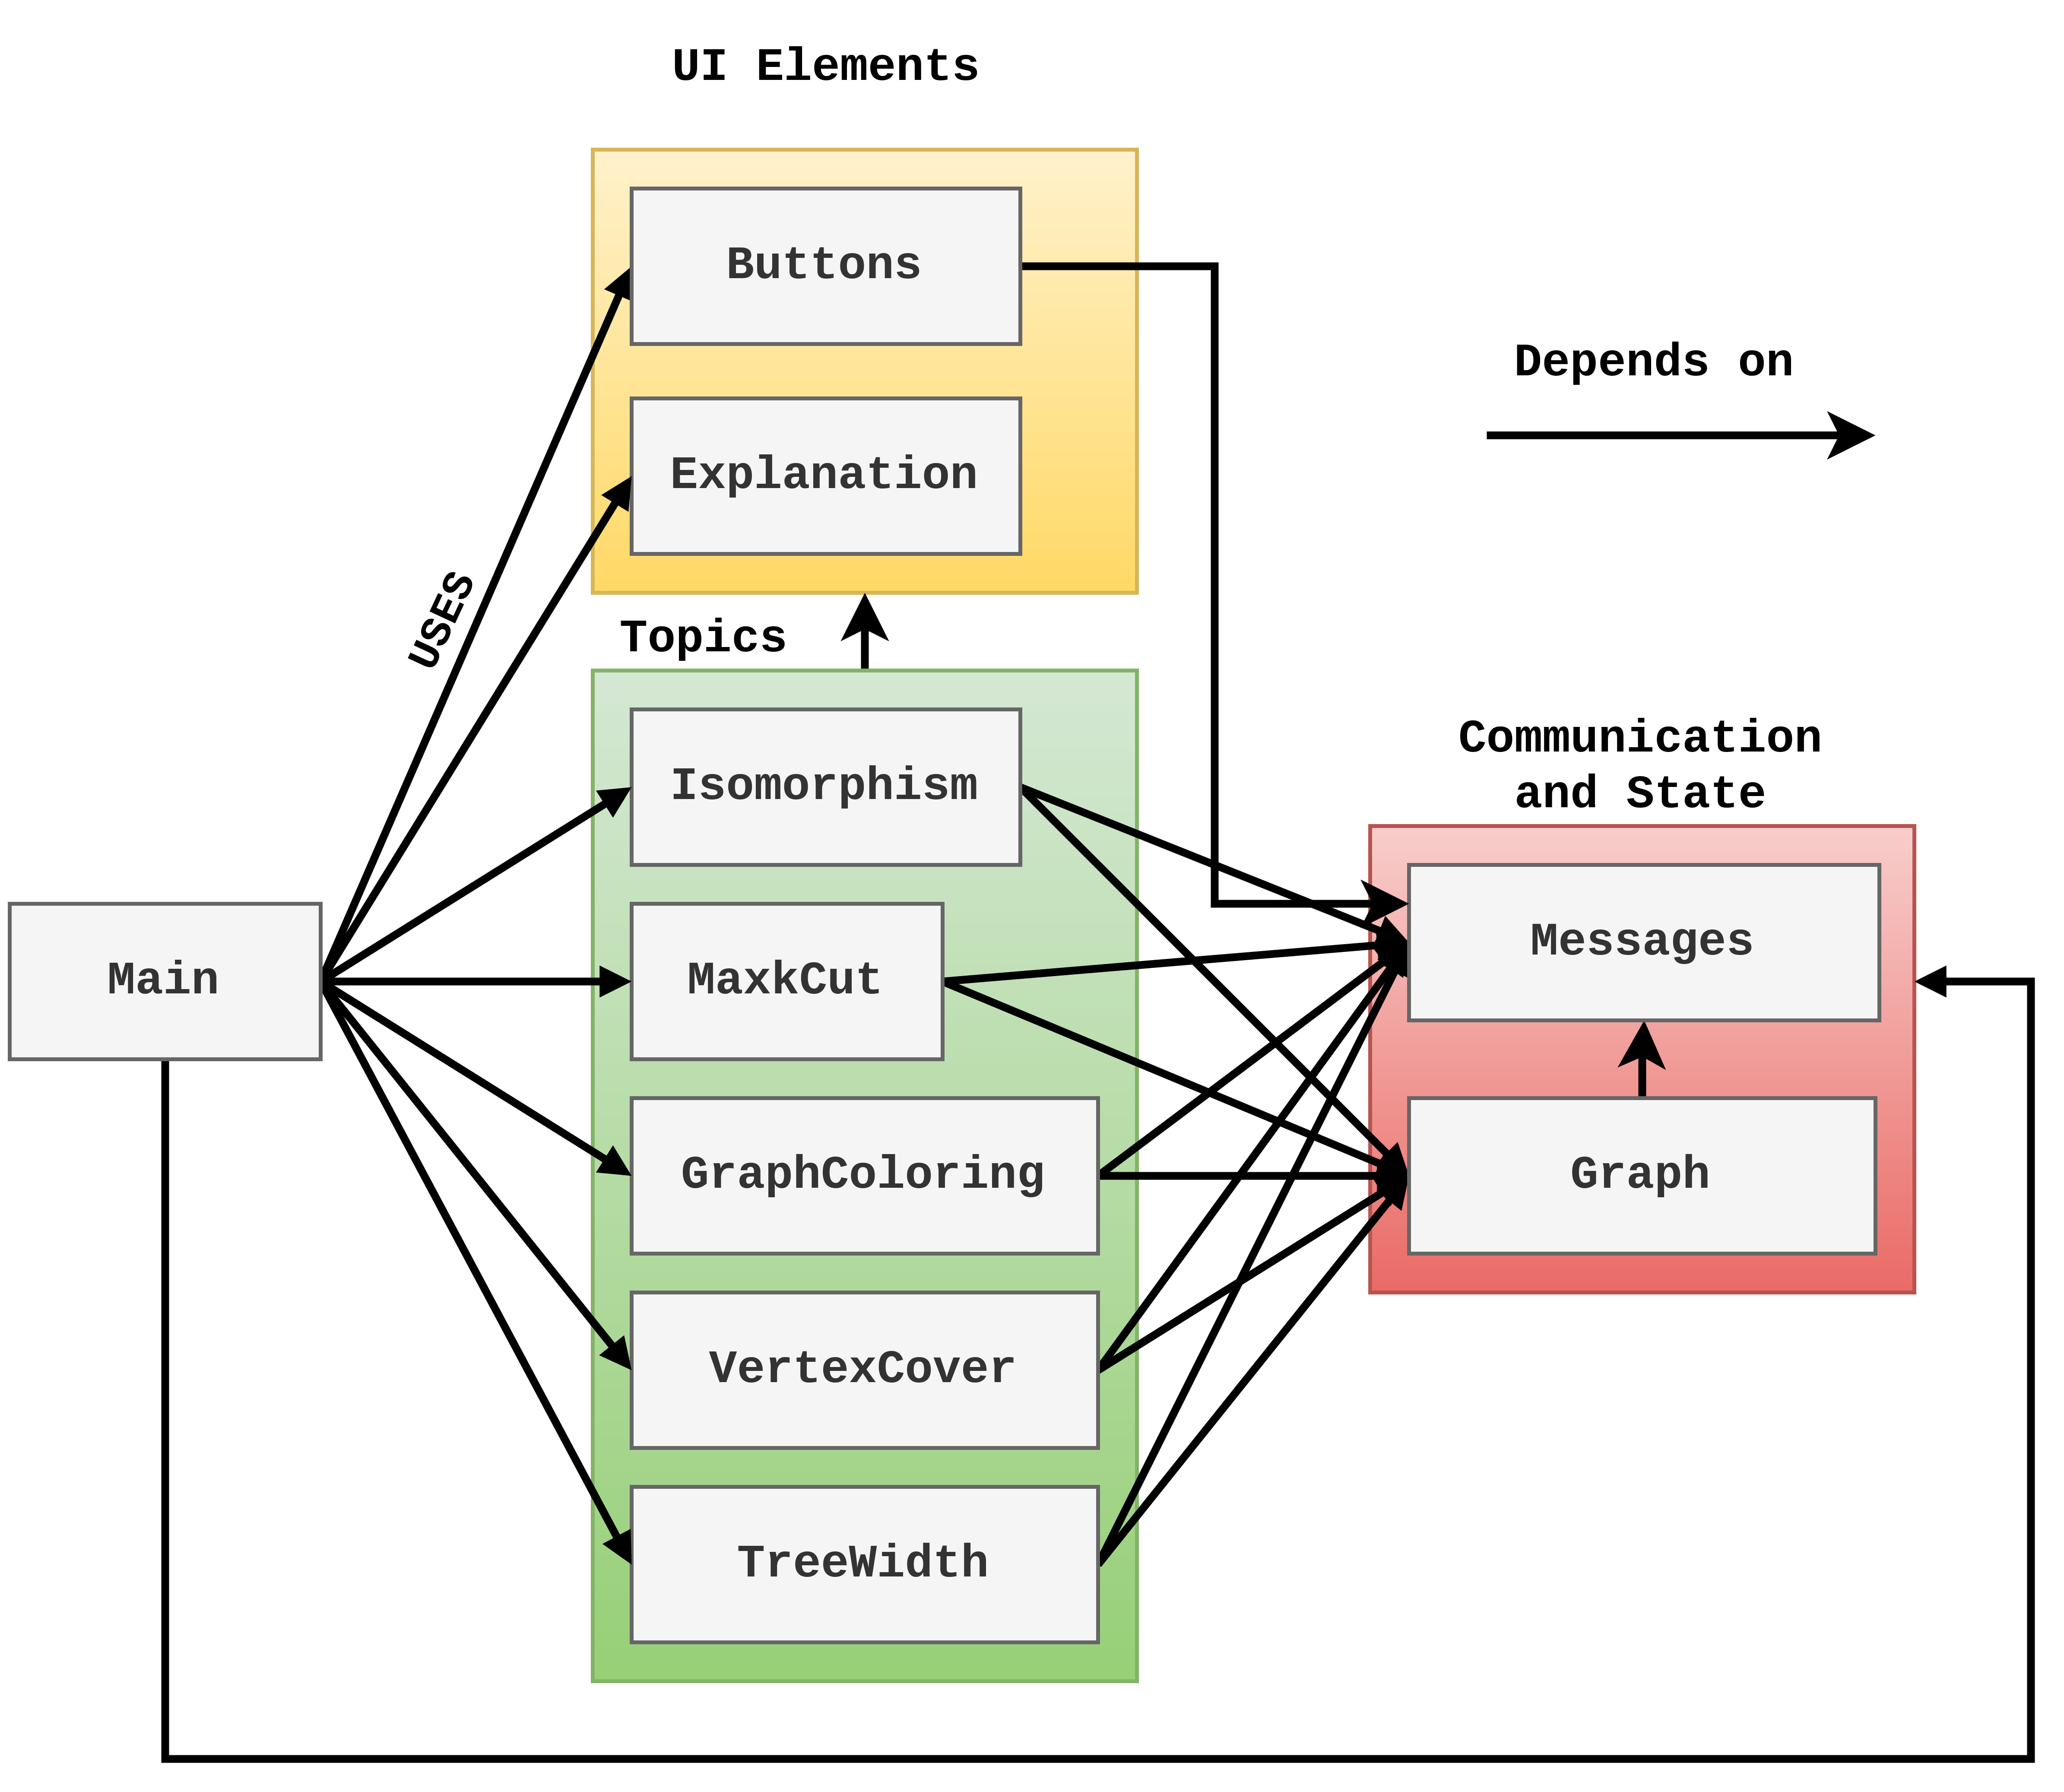
\includegraphics[width=4.22in]{Modules}
\caption{
        Modules in the Program. Arrows from the blunt end to
        the pointy end depict dependency.
        }
\end{figure}

\section{Software Engineering Practices}
In the following subsections, how a few good practices which were adopted to
make the project of this size manageable and organized are explained.

\subsection{Version Control}
The program along with the documentation and the dissertation report were
version controlled in a single GitHub repository. A git repository, gives the
developer confidence for fearless refactoring and feature enhancement by the
way of creating separate branches for separate issues. Therefore a different
branch was created for editing documentation, and it was made sure that
modification in code files was not done on this branch. Similarly, a branch for
code refactoring didn't modify the documentation part hence separating
concerns.  Furthermore a branch was conveniently discarded if an adventure in a
radical change in code went wrong.

\subsection{Continuous Deployment}
The web application concerning the project is deployed on the World Wide Web
using Netlify. It is a service which lets one host a front end website. It is
connected to the master branch of the GitHub repository of the project. Every
time a new version is pushed to the master, netlify service fetches the new
version of the app from the repository, builds it according to the build script
present in the GitHub repository and deploys the web application on a specific
URL. The build and deployment can also be done manually by going to the
dashboard of the Netlify website. The build and deployment process primarily
consists of running a script to transpile Elm code to a JavaScript file and copy
the output along with the boiler plate HTML to the publish directory.

If it is needed to deploy the application anew instantaneously (something which
is required to test the website for different screen sizes) a \emph{curl}
command with a specific URL called a \emph{build hook} is executed on the local
machine.  It deployes the website from the code in the master branch in the
repository.


\subsection{Documentation}
Documentation for the project was done in a continuous fashion in a variety of
ways, such as a wiki for code implementation and a guide for future work, time
logging for project management and report writing for the submission. 

The wiki was informed heavily from the code comments made to explain the
functions. Time logging brought a sense of discipline in the whole endeavor.
It also helped in estimating time required to complete the tasks which lay in
future and asses the learning curve.
